\documentclass[12pt, twoside]{article}
\usepackage[letterpaper, margin=1in, head=30pt, headsep=0.1in]{geometry}
\usepackage[english]{babel}
\usepackage[utf8]{inputenc}
\usepackage{amsmath}
\usepackage{amsfonts}
\usepackage{amssymb}
\usepackage{tikz}
\usetikzlibrary{quotes, angles}

\usepackage{graphicx}
\usepackage{enumitem}
\usepackage{multicol}

%\usepackage{pgfplots}
%\pgfplotsset{width=10cm,compat=1.9}
%\usepgfplotslibrary{statistics}
%\usepackage{pgfplotstable}
%\usepackage{tkz-fct}
%\usepackage{venndiagram}

\usepackage{fancyhdr}
\pagestyle{fancy}
\fancyhf{}
\renewcommand{\headrulewidth}{0pt} % disable the underline of the header
\raggedbottom
\newif\ifmeta
\metatrue %print standards and topics tags

\title{Math AI Worksheet Generator and Formative Assessment System}
\author{Chris Huson}
\date{December 2020}

%\fancyhead[RE]{\thepage}
%\fancyhead[RO]{\thepage \\ Name: \hspace{3cm}}
%\fancyhead[L]{BECA / Dr. Huson / 10th Grade Geometry\\* 7 June 2019}
%
%\begin{document}
%\subsubsection*{13.7 Homework: Cross sections, distance applications}
%\fancyhead[L]{BECA / Dr. Huson / Geometry 03-Volume+angle-bisectors\\* pset ID: 34}

\begin{document}

\subsubsection*{4.8 Quiz Transformations}
\begin{enumerate}

\item A translation maps $A$ to $A'$, as shown, $A(3,1) \rightarrow A'(6,3)$.
\begin{multicols}{2}
  \begin{enumerate}
    \item What is the horizontal shift, how many squares right or left? \vspace{1.25cm}
    \item What is the vertical shift, how many squares up or down? \vspace{1.25cm}
    \item Apply the same translation to $C(1,3)\rightarrow C'(x,y)$. On the grid, mark and label the point $C'$ as an ordered pair.
    \end{enumerate}
    \begin{flushright}
    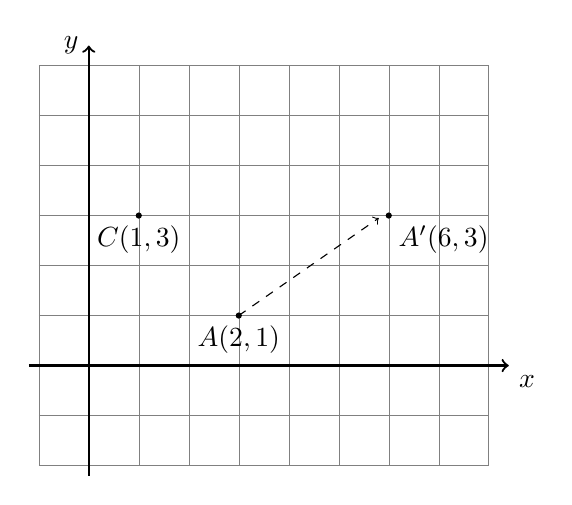
\begin{tikzpicture}[scale=.635]
      \draw [help lines] (-1,-2) grid (8,6);
      \draw [thick, ->] (-1.2,0) -- (8.4,0) node [below right] {$x$};
      \draw [thick, ->] (0,-2.2)--(0,6.4) node [left] {$y$};
      \draw [fill] (3,1) circle [radius=0.05] node[below] {$A(2,1)$};
      \draw [fill] (6,3) circle [radius=0.05] node[below right] {$A'(6,3)$};
      \draw [->, dashed] (3,1)--(5.8,2.95);
      \draw [fill] (1,3) circle [radius=0.05] node[below] {$C(1,3)$};
    \end{tikzpicture}
    \end{flushright}
\end{multicols}

\newpage
\item A translation maps triangle $ABC$ onto triangle $DEF$. \\[0.5cm]
Fill in the blank with each corresponding object. \vspace{0.5cm}
    \begin{multicols}{2}
      \begin{tikzpicture}[scale=1]
        \coordinate [label=above left:$A$](A) at (95:2);
        \coordinate [label=below:$B$](B) at (0, 0);
        \coordinate [label=right:$C$](C) at (25:3.5);
        \draw [thick] (A)--(B)--(C)--cycle;
        \draw [thick, xshift=2cm, yshift=-3cm] (95:2) node[left]{$D$}--
        (0,0) node[below]{$E$}--
        (25:3.5) node[right]{$F$}--cycle;
      \end{tikzpicture}

      \begin{enumerate}
        \item $A \rightarrow$ \rule{2cm}{0.15mm}
        \item $\angle B \cong$ \rule{2cm}{0.15mm}
        \item $\overline {AB} \cong$ \rule{2cm}{0.15mm}
        \item Which statement best justifies $\triangle ABC \cong \triangle DEF$? \\[0.5cm]
        Since translation is a rigid motion, the triangle's size and shape remains the same.\\[0.5cm]
        A dilation centered at point $A$ with a scale factor $k=2$ was performed.
      \end{enumerate}
    \end{multicols}

\newpage
\item A translation maps $P(3,5) \rightarrow P'(2,9)$. What is the image of $Q(-3,2)$ under the same translation?

\newpage
\item Translate $\triangle ABC$ by $(x,y) \rightarrow (x+4, y-1)$. Make a table of the coordinates and plot and label the image on the axes.
  \begin{flushright}
    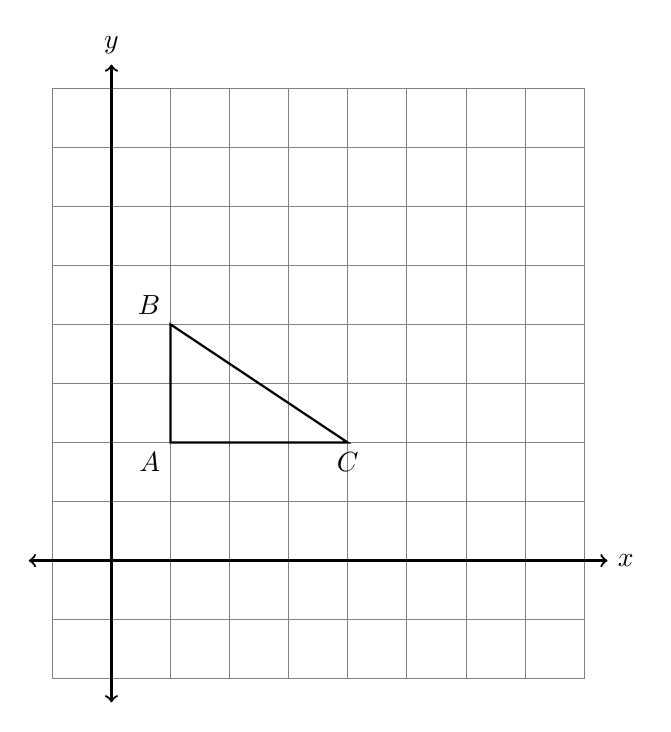
\begin{tikzpicture}[scale=.75]
    \draw [help lines] (-1,-2) grid (8,8);
    \draw [thick, <->] (-1.4,0) -- (8.4,0) node [right] {$x$};
    \draw [thick, <->] (0,-2.4)--(0,8.4) node [above] {$y$};  
    \draw [thick]
      (1,2) node[below left] {$A$}--
      (1,4) node[above left] {$B$}--
      (4,2) node[below] {$C$}--cycle;  
    \end{tikzpicture}
  \end{flushright}

\newpage
\item A dilation centered at $A$ with scale factor $k=2$ maps $\triangle ABC \rightarrow \triangle ADE$. Given the sides of the preimage, $AC = 10$, $BC = 7$, $AB = 12$. \\[0.5cm]
$DE = 14$, how long are $AD$ and $AE$?
    \begin{flushright}
      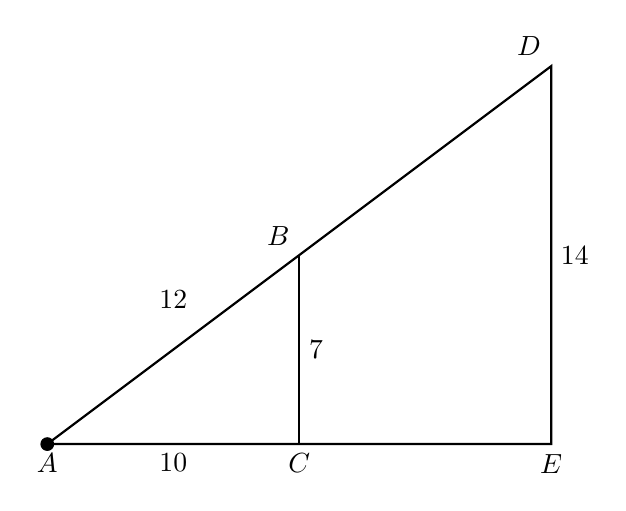
\begin{tikzpicture}[scale=0.8]
        \draw [-, thick] (0,0)--
        (8,0) node[below]{$E$}--
        (8,6) node[above left]{$D$}--cycle;
        \draw [thick] (4,0)--(4,3);
        \draw [fill] (0,0) circle [radius=0.1] node[below] {$A$};
        \node at (4,0) [below]{$C$};
        \node at (4,3) [above left]{$B$};
        \node at (2, 0) [below]{$10$};
        \node at (2, 2) [above]{$12$};
        \node at (8, 3) [right]{$14$};
        \node at (4, 1.5) [right]{$7$};
      \end{tikzpicture}
    \end{flushright}

\newpage
\item Dilate $\triangle ABC \rightarrow \triangle A'B'C'$ by a factor of $k=1.5$ centered at the origin,\\
$(x,y) \rightarrow (1.5x, 1.5y)$. Plot and label the image on the axes. Make a table of the vertices and their coordinates.
\begin{flushright}
    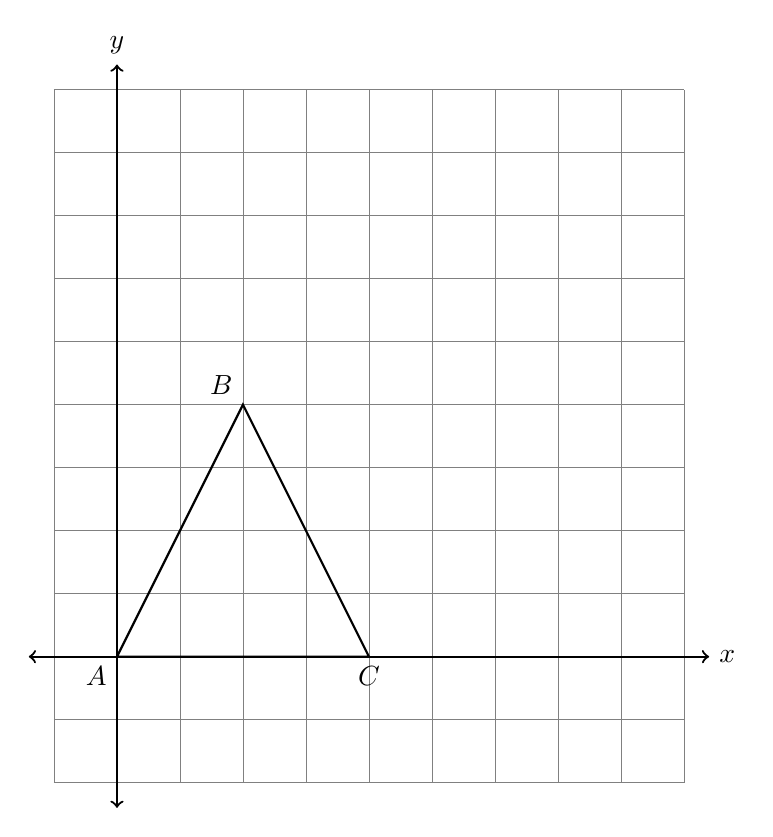
\begin{tikzpicture}[scale=0.8]
    \draw [help lines] (-1,-2) grid (9,9);
    \draw [thick, <->] (-1.4,0) -- (9.4,0) node [right] {$x$};
    \draw [thick, <->] (0,-2.4)--(0,9.4) node [above] {$y$};  
    \draw [thick]
      (0,0) node[below left] {$A$}--
      (2,4) node[above left] {$B$}--
      (4,0) node[below] {$C$}--cycle;  
  \end{tikzpicture}
\end{flushright}

\newpage
\item A transformation is performed on a parallelogram, $MATH \rightarrow M'A'T'H'$, as shown in the diagram. \\[0.5cm]
What is the transformation? (Hint: Is it a translation, reflection, rotation, or dilation? What is its center? What is the scale factor, $k$?)
\begin{flushright}
    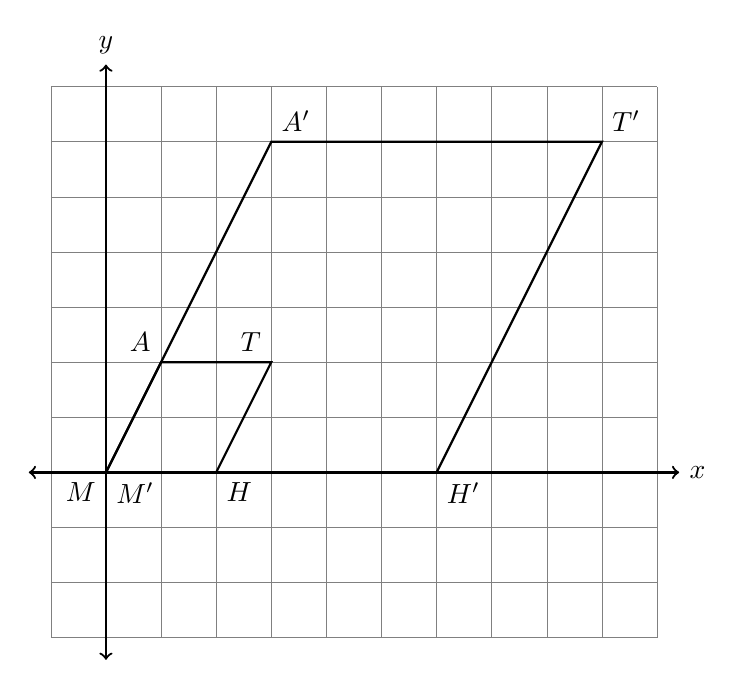
\begin{tikzpicture}[scale=0.7]
    \draw [help lines] (-1,-3) grid (10,7);
    \draw [thick, <->] (-1.4,0) -- (10.4,0) node [right] {$x$};
    \draw [thick, <->] (0,-3.4)--(0,7.4) node [above] {$y$};  
    \draw [thick]
      (0,0) node[below left] {$M$}--
      (1,2) node[above left] {$A$}--
      (3,2) node[above left] {$T$}--
      (2,0) node[below right] {$H$}--cycle;
    \draw [thick]
      (0,0) node[below right] {$M'$}--
      (3,6) node[above right] {$A'$}--
      (9,6) node[above right] {$T'$}--
      (6,0) node[below right] {$H'$}--cycle;
  \end{tikzpicture}
\end{flushright}

\newpage
\item Dilate $\triangle ABC \rightarrow \triangle A'B'C'$ by a factor of $k=2.5$ centered at the origin, \\
$(x,y) \rightarrow (2.5x, 2.5y)$. Plot and label the image on the axes. (table optional)
\begin{flushright}
    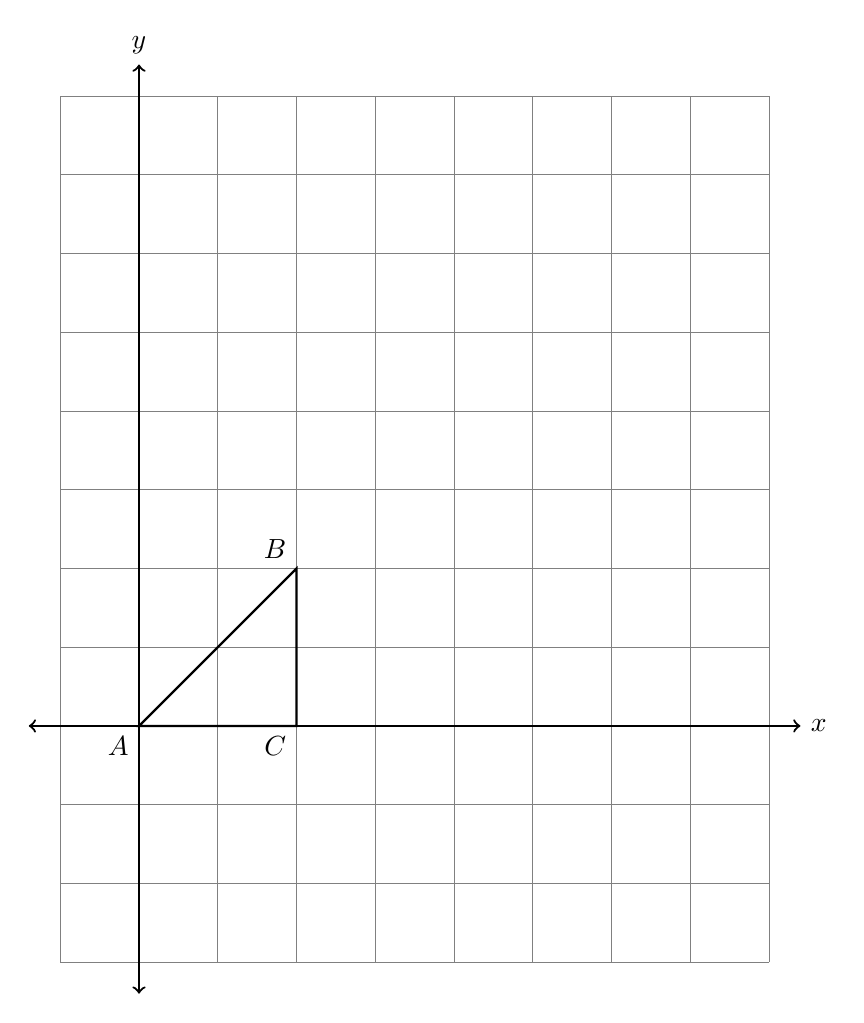
\begin{tikzpicture}[scale=1]
    \draw [help lines] (-1,-3) grid (8,8);
    \draw [thick, <->] (-1.4,0) -- (8.4,0) node [right] {$x$};
    \draw [thick, <->] (0,-3.4)--(0,8.4) node [above] {$y$};  
    \draw [thick]
      (0,0) node[below left] {$A$}--
      (2,2) node[above left] {$B$}--
      (2, 0) node[below left] {$C$}--cycle;  
  \end{tikzpicture}
\end{flushright}

\end{enumerate}
\end{document}